\chapter{Conception du système}

\section{Introduction}
%Of course talk here about what the chapter is about
\paragraph{}
Durant ce chapitre, nous allons présenter en détail les étapes de conceptions de notre système, tout d'abord une architecture générale est présentée et décortiquée, ensuite chaque module du système sera détaillé du point de vue des composants qui le constitueraient en donnant un maximum de détails tout en restant assez concis. Une conclusion viendra clôturer ce chapitre pour introduire ensuite le suivant.
\section{Architecture du système}
%Try to be as precise as possible while letting room for more details to the next sections
\begin{figure}[H]
	\centering
	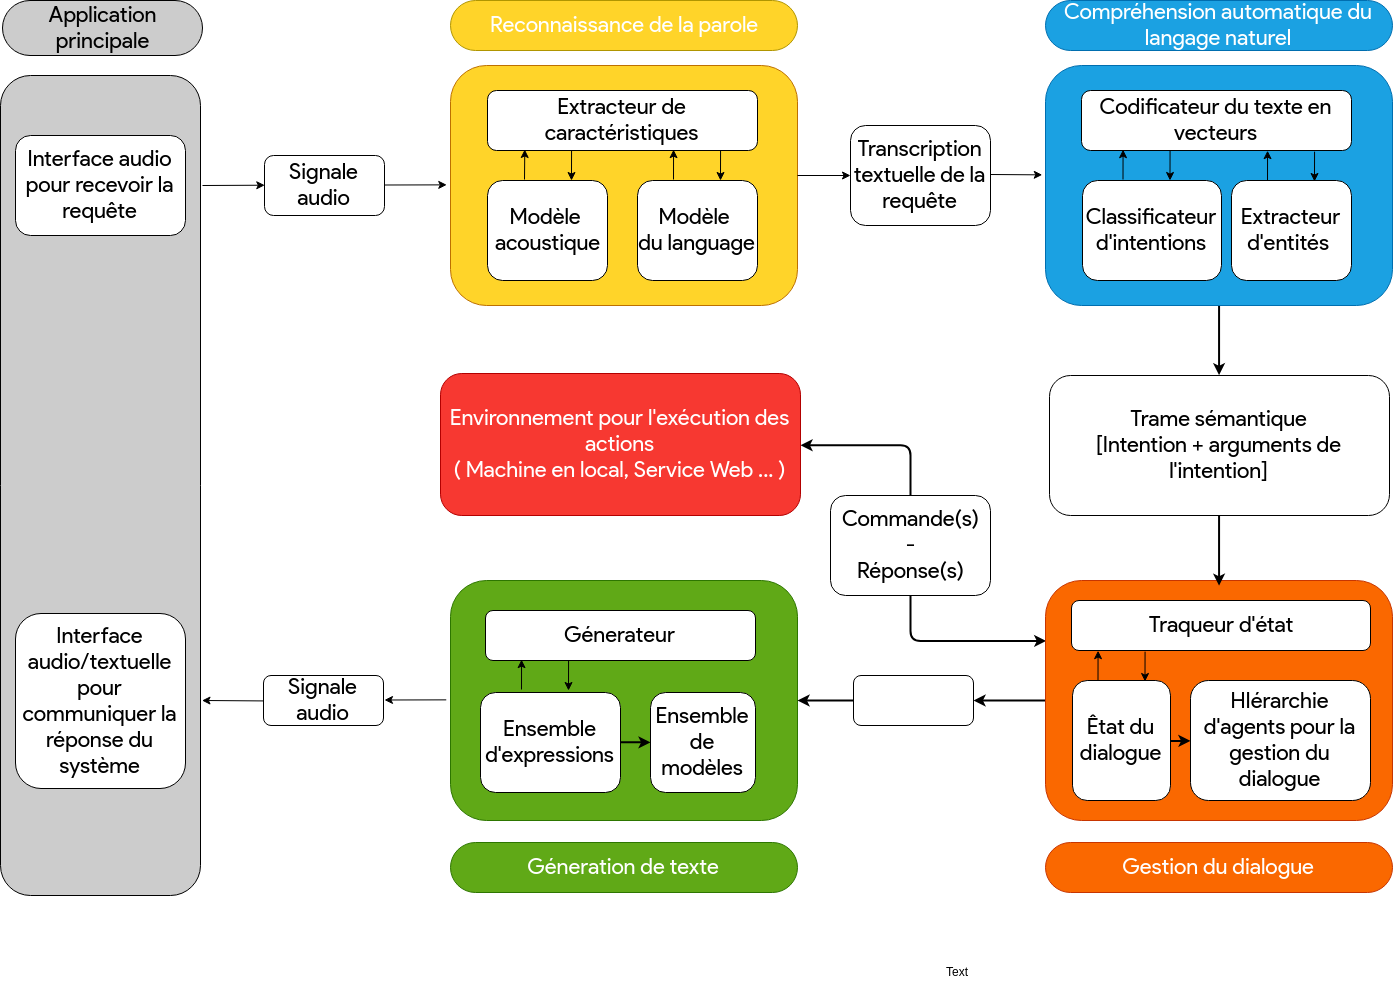
\includegraphics[width=0.87\linewidth]{images/SPA_architecture.png}
	\caption{Architecture générale de notre système}
	\label{spaArch}
\end{figure}
\paragraph{}
Comme montré dans la figure ci dessus (voir ~\ref{spaArch}) et comme cité dans le chapitre précédent (voir \ref{spaSchemSection}) le système se présente comme l'interconnexion de cinq parties dont une interface \footnote{Ici nous par interface nous entendons le sens abstrait du terme et non obligatoirement le sens interface graphique} et quatre modules internes, chaque module forme ainsi un maillon d'une chaîne qui représente une partie du cycle de vie du système. L'architecture du système est une pipeline (chaîne de traitement) de processus qui s'exécutent de manière indépendante mais qui font circuler un flux de données entre eux dans un format préalablement décidé (voir ~\ref{fig:spaDiagram}). Nous pouvons séparer ces parties en deux catégories :
	\subsection{Couche utilisateur}
%	What the users sees as input/output and the interfaces that are available for him
	\paragraph{}
	Cette couche représente ce que l'utilisateur peut voir comme entrée/sortie et les interfaces qui lui sont accessibles, puisque l'assistant est un processus qui communique majoritairement avec l'utilisateur à travers des échanges verbaux, nous avons pensé à implémenter l'interface du système comme une processus qui s'exécute en arrière plan et qui attend d'être activer (pour le moment par un événement physique, c.à.d clique sur un bouton/icône ou raccourci clavier), l'assistant pourra ensuite répondre en affichant un texte à l'écran qui sera vocalement synthétisé envoyer à l'utilisateur via l'interface de sortie de son choix (afficher le texte et sa transcription vocale pourrait palier au manque d'un périphérique de sortie audio).
	\subsection{Couche système}
	
%	What the users doesn't see and what are the main components of the system
	\paragraph{}
	\label{system_layer}
	Cette couche quant à elle représente ce que l'utilisateur ne voit pas et fait donc partie du fonctionnement interne du système, elle regroupe les quatre grandes étapes d'un cycle de vie pour une commande reçu de la couche utilisateur. Comme mentionné dans le chapitre précédent (voir \ref{spaLifeCycle}), la requête passe par un module de reconnaissance de la parole, qui traduira en texte le signale audio correspondant à la requête, le module suivant va extraire l'intention de l'utilisateur et ses arguments (par exemple \textit{"open the home folder"} pourrait donner  une intention dy type  \textit{open\_file\_desire[file\_name="home",parent\_directory="?"]}), le gestionnaire de dialogue gardera trace de l'ensemble des échanges effectués entre l'utilisateur et l'assistant et essayera d'atteindre le but final formuler par la requête (la plus récente ou la plus ancienne), pour ce faire il aura besoin d'interagir avec ce qu'on a appelé un environnement d'exécution, qui peut être la machine où l'assistant réside ou une API \footnote{Application programming interface ou interface de programmation applicative } qui aura accès à un service a distance (sur internet par exemple) ou locale (dans un réseau domestique). Finalement une action spéciale qui servira à informer l'utilisateur sera envoyé au module suivant pour être transformé en son équivalant en langage naturel, puis le texte sera vocalement synthétiser et envoyé vers l'interface de sortie de l'application.
	
	\paragraph{}
	Nous allons maintenant détailler la conception des différents modules en précisant à chaque fois le ou les processus de sa mise en œuvre. 
\section{Module de reconnaissance automatique de la parole}
\paragraph{}
Premier module du système, il joue un rôle clé dans la véridicité du dialogue entre l'utilisateur et la machine, en effet il devait être assez robuste et précise dans la transcription de la requête en entrée minimiser les erreurs et les ambiguïtés qui peuvent survenir dans le reste de la pipeline. C'est pour cela que nous avons décidé de ne pas développer un sous-système en partant de zéro, par faute de temps et par soucis de précision nous avons décidé de nous baser sur un outil open-source nommé DeepSpeech \cite{deepspeech_paper}, naturellement du fait que ce soit un projet open-source nous avons pu avoir accès à différentes informations concernant le modèle d'apprentissage, d'inférence et la nature des données utilisé pour le premier et le teste du deuxième.
	\subsection{Architecture du module}
	\paragraph{}
	Le module possède une architecture en pipeline dont chaque composant exécute un traitement sur la donnée reçu par son prédécesseur
	\begin{figure}[H] 
		\centering
		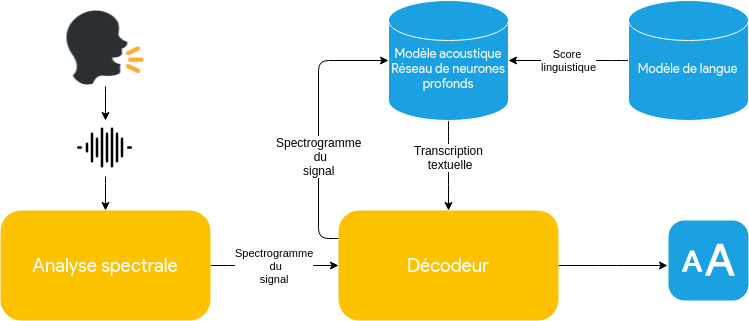
\includegraphics[width=0.88\linewidth]{images/Conception/ASR/schema.png}
		\caption{Architecture de notre module de reconnaissance de la parole}
	\end{figure}
	\subsection{Modèle acoustique}
		\subsubsection*{Type du modèle}
		\paragraph{}
		Le modèle d'apprentissage (qui est principalement le modèle acoustique à l'exception d'une partie consacré au modèle linguistique) possède une architecture en réseau de neurones avec apprentissage de bout-en-bout composé de trois parties : 
		\begin{itemize}
			\item Deux couches de convolution spatiale : pour capturer les patrons dans la séquence du spectrogramme du signal audio.
			\item Sept couches de récurrence (Réseaux de neurones récurrents) pour analyser la séquence de patrons (ou caractéristiques) engendré par les couches de convolutions. 
			\item Une couche de prédiction utilisant un réseau de neurone complètement connecté pour prédire le caractère correspondant à la fenêtre d'observation du spectrogramme du signal audio. La fonction d'erreur prend en compte la similarité du caractère produit avec le véritable caractère ainsi que la vraisemblance de la séquence produite par rapport à un modèle de langue basé sur les N-grammes (voir \ref{n-grams})
		\end{itemize}
		\begin{figure}[H] 
			\centering
			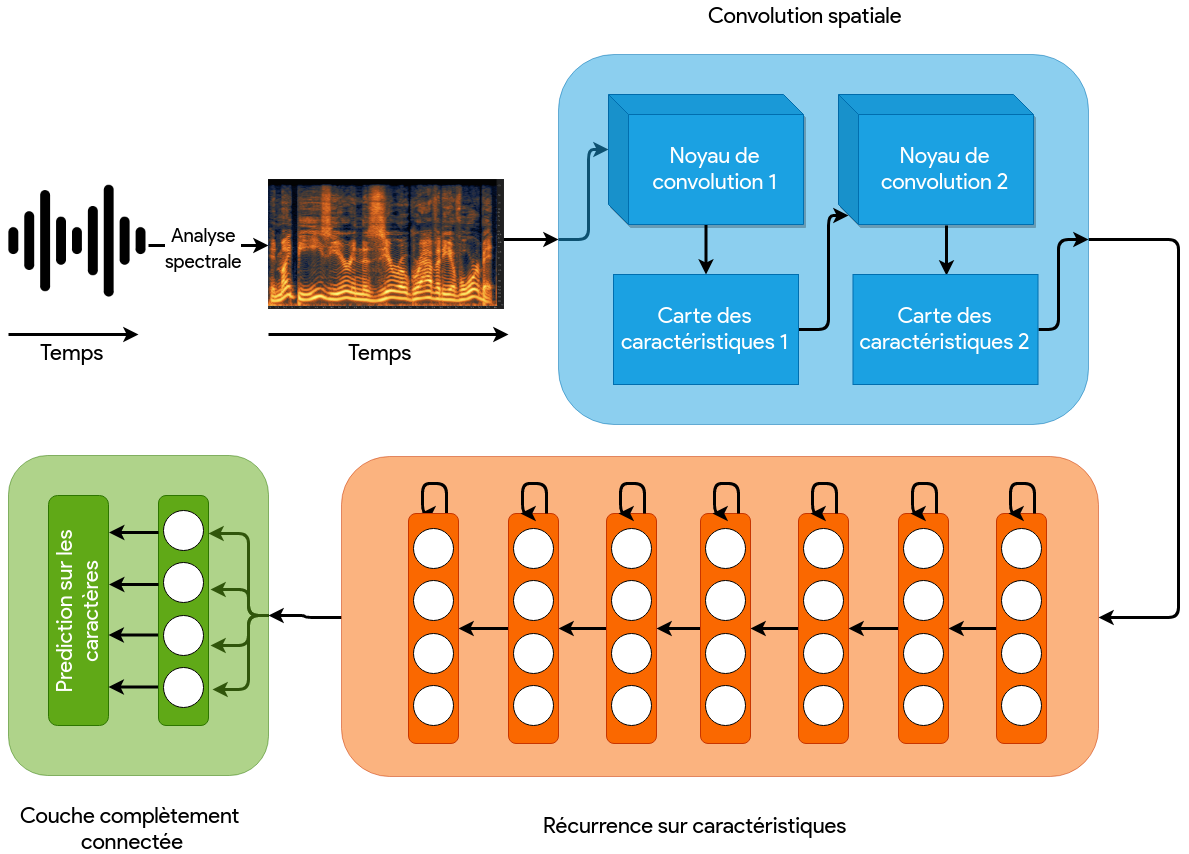
\includegraphics[width=0.88\linewidth]{images/Conception/ASR/deeps_speech_arch.png}
			\caption{Architecture du modèle DeepSpeech \cite{deepspeech_paper}}
			\label{fig:deepSpeechArch}
			
		\end{figure}
		\subsubsection*{Données d'apprentissage}
%		audio files and their transcriptions
		\paragraph{}
		Pour entraîner le modèle acoustique, Mozilla à lancé le projet Common Voice  \footnote{\url{https://voice.mozilla.org/fr}} une plateforme enligne pour récolter des échantillons d'audio avec leurs transcriptions textuelles, chaque lot (batch) de données reçu est alors manuellement validé par l'équipe de Mozilla pour l'inclure dans la banque de données d'exemples. À ce jour plus et pour la langue anglaise, la plateforme à récolté plus de 22Go de données, soit 803 heures d'enregistrement appartement à plus de 30 000 voix différentes dont 582 heures ont été validées. Mais ces données ne sont rien comparées à celle déjà utilisées pour l'apprentissage initial, en effet plusieurs source ont été combinées pour construire cet ensemble de données, dans \cite{deepspeech_paper} il a été mentionné que trois ensembles d'apprentissage existants ont étés utilisés dont WSJ (Wall Stret Journal) \footnote{\url{http://www.cstr.ed.ac.uk/corpora/MC-WSJ-AV/}}, Switchboard \footnote{\url{https://catalog.ldc.upenn.edu/LDC97S62}} et Fisher \footnote{\url{https://catalog.ldc.upenn.edu/LDC2004S13}} qui cumulent 2380 heures d'enregistrements audio en anglais et plus de 27 000 voix différentes, vient s'ajouter à cela l'ensemble Baidu \footnote{\url{https://ai.baidu.com/broad/introduction}} avec 5000 heures d'enregistrements et 9600 locuteurs.
		
	\subsection{Modèle de la langue}
		\subsubsection*{Type du modèle}
		\paragraph{}
		Pour ce qui est du type du modèle de langue, c'est un modèle basé sur les N-grammes (3-grammes pour être plus précis) qui est utilisé, en effet il permet de façon assez simple et intuitive de capturer l'enchaînement des mots dans une langue donnée, rendant ainsi la transcription assez proche de la façon dont les mots sont distribués dans le corpus d'apprentissage.
		
		\subsubsection*{Données d'apprentissage}
		\paragraph{}
		À l'origine, DeepSpeech utilise un modèle de langue dont la source n'est pas dévoilée par les chercheurs dans \cite{deepspeech_paper}, mais son volume est approximativement de 220 million de phrases avec 495 000 mots différents. Cependant puisque ce corpus nous reste inconnu et qu'il a probablement été construit pour reconnaître des séquence de mots de phrase en anglais assez générales, nous avons décidé de construire notre propre modèle de langue en récoltant des données depuis des dépôts sur le site \href{https://github.com/}{Github}, plus précisément les fichiers README.md des dépôts qui font office de manuels d'utilisation d'un projet hébergé sur le site, ce type de fichier renferment généralement des instructions de manipulation de fichiers, de lancement de commandes ..., ce qui offre un bon corpus pour le modèle de langue, car en effet notre système se concentre plus sur l'aspect de manipulation d'un ordinateur, donc la probabilité de trouver certaines séquences de mots qui appartiennent au domaine du Tech est plus élevé en théorie. La procédure suivi est la suivante : 
		\begin{figure}[H] 
			\label{lm_gathering}
			\centering
			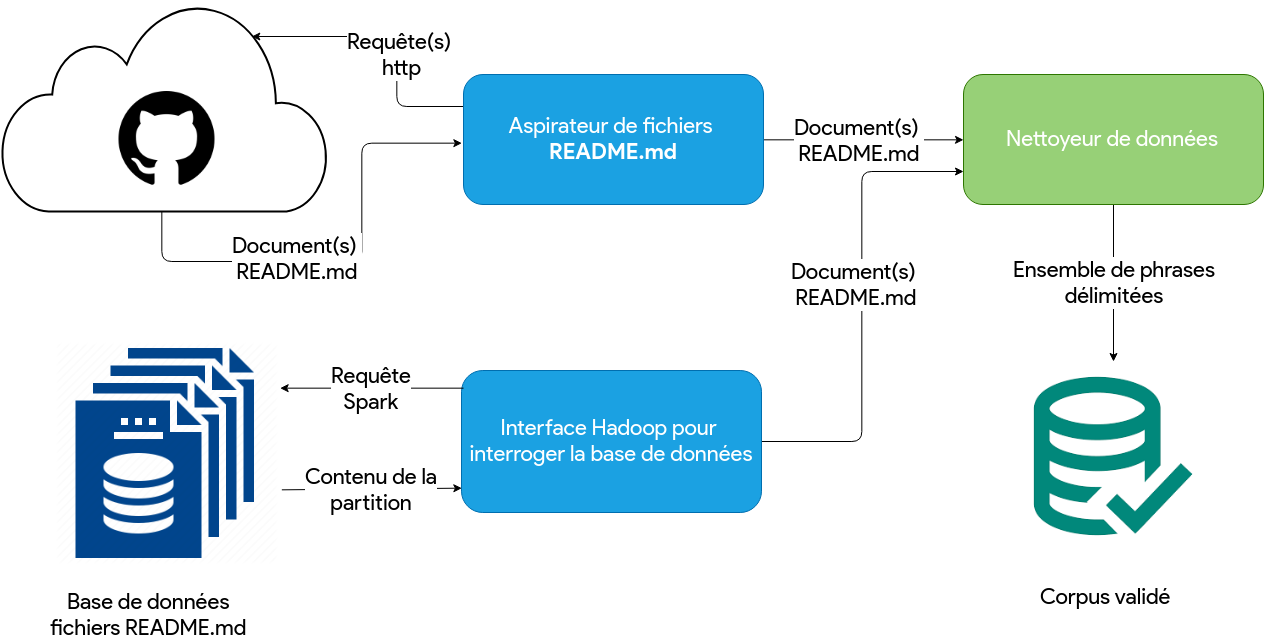
\includegraphics[width=0.88\linewidth]{images/Conception/ASR/lm_gathering.png}
			\caption{Processus de génération du corpus pour le modèle de langue}
		\end{figure}
		\newpage
		\begin{itemize}
			\item L'acquisition des données dans leur format brut \textbf{.md} (markdown) se fait de deux manières :
			\begin{itemize}
				\item Depuis le site officiel de GitHub en faisant des requêtes http au serveur en suivant le patron suivant des urls : 
				\begin{lstlisting}[language=python]
				'http://raw.githubusercontent.com/'+NOM_DÉPOT+'/master/README.md'\end{lstlisting}
				La liste des noms de dépôt est disponible dans un fichier \footnote{\url{https://data.world/vmarkovtsev/github-readme-files/file/top_broken.tsv}} en free open acces au format \textbf{.csv} dont les colonnes sont \textit{Nom\_Utilisateur} et \textit{Nom\_Dépot} 
				\item En lisant un base de 16 millions de fichiers différents dont la taille totale atteint 4.5 Go  
			\end{itemize}
			\item Les deux sources de données envoient ensuite les fichiers récoltés au nettoyeur de fichiers pour en extraire seulement les parties qui ont du sens (c.à.d paragraphes, titres, instructions ...).
			\item Le corpus final est ensuite construit à partir des paragraphes extraits à l'étape précédente après les avoir segmenté en phrases (en utilisant un modèle de segmentation prédéfini) donnant le format suivant \begin{lstlisting}[language=xml]
			<s>Phrase1</s>
			<s>Phrase2</s>
			...
			<s>PhraseN</s>\end{lstlisting}
		\end{itemize}
		

\section{Module de compréhension automatique du langage naturel}
\paragraph{}
Second module du système, son rôle et de faire office de couche d'abstraction entre la requête de l'utilisateur formulée dans un langage naturel et le fonctionnement interne du système qui lui comprend (et parle) un langage plus formel, on parle ici de la construction d'un représentation sémantique de la requête. Pour ce faire nous avons opté pour l'approche par apprentissage automatique, compte tenu des bons résultats obtenus par certaines architectures \cite{intent_slots},\cite{intent_classification} et ceux malgré le petit de nombre de données d'apprentissage, cette option nous paru plus abordable que la construction d'un analyseur basé sur règles, qui sont souvent assez rigide.
	\subsection{Architecture du module}
	\begin{figure}[H] 
		\label{nlu_arch}
		\centering
		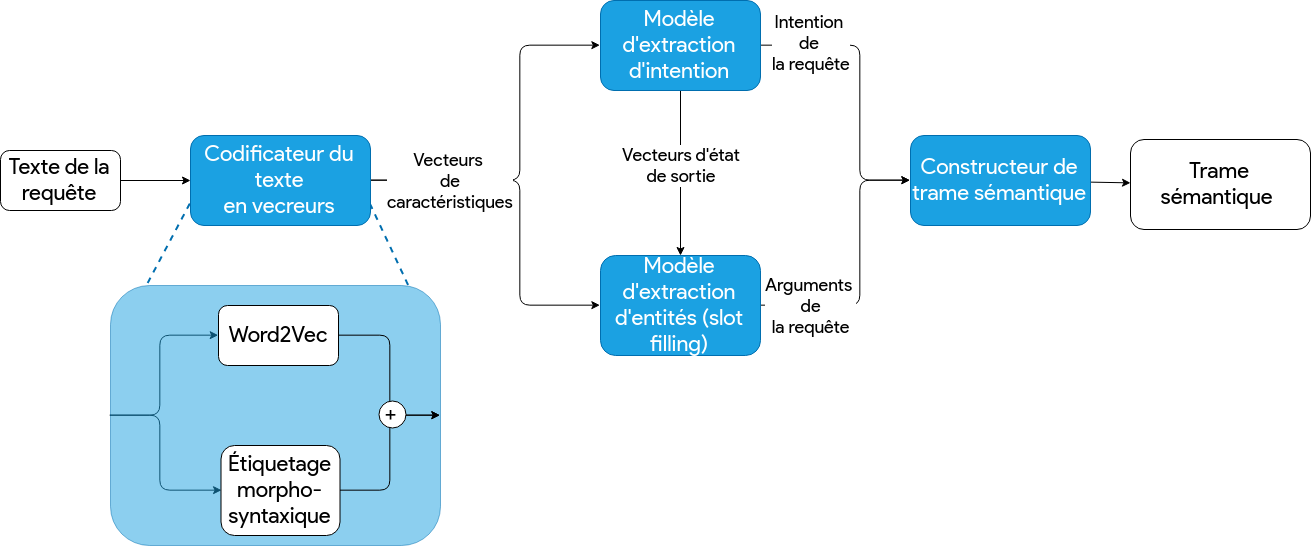
\includegraphics[width=0.88\linewidth]{images/Conception/NLU/nlu_module_arch.png}
		\caption{Architecture du module  compréhension automatique du langage naturel}
	\end{figure}
	\paragraph{}
	Comme précédemment cité (voir \ref{system_layer}), le module possède une architecture en pipeline qui reçoit en entrée le texte brut de la requête, sa codification varie selon les approches que nous avons exploré et qui seront plus expliciter dans le chapitre suivant Réalisation et Expérimentions, pour mieux capturer l'aspect sémantique des mots dans le texte, nous avons décidé d'utiliser un modèle pré-entraîné par Google de Word2Vec (entraîné sur 100 milliard de mots) pour produire un vecteur de taille fixe pour chaque mots, pour encoder l'information syntaxique de la requête nous avons concaténé au vecteur de prolongement de chaque mot de la requête (Word Embedding Vector) le vecteur codifiant son étiquette morphosyntaxique. Après avoir codifié la séquence de mots, elle est envoyée aux modèles de classification d'intentions et d'extraction d'entités \footnote{Par entité nous entendons les arguments de l'intention}, qui sont en fait un seul modèle joint dont l'architecture est détailler dans \ref{joint_model}. Ces deux informations sont ensuite décodées et passées au constructeur de trame sémantique qui structurera ces dernières en une seule entité sémantique dans le format suivant : 
	donnant le format suivant \begin{lstlisting}[language=json]
	{
		intent  : "open_file_desire",
		entities : [
			{	
				entity	: "string",
				name	: "file_name",
				value	: "tes.py",
				start	: "31",
				end		: "37",
			}
		]
	}
	\end{lstlisting}
	
%	\subsection{Analyse sémantique basée sur les grammaires de dépendances}
	\subsection{Analyse sémantique avec apprentissage automatique}
		\subsubsection{Modèle(s) utilisé}
		\paragraph{}\label{joint_model}
		Comme vu dans le chapitre précédent (voir \ref{nlu_chap2}) l'architecture adopté est une architecture mono-entrée/multi-sorties dont l'entrée est une séquence de mots codifiés et les sorties sont une séquence d'étiquettes et une classe associé au texte. Nous pouvons distingué les deux parties qui sont l'encodage et le décodage de la séquence, l'encodage sert à la fois à l'attribution de la classe (l'intention) et à l'initialisation de la séquence de décodage (pour l'attribution de son étiquette à chaque mot).
		\par
		L'encodage se fait en utilisant un réseau de neurones récurent de type BLSTM (Bidirectionnel Long Short Term Memory) pour mieux capturer le contexte droit (respectivement gauche) de chaque entrée, le dernier vecteur en sortie est ensuite utilisé comme vecteur d'entrée pour un réseau de neurones Fully Connected (Complètement connecté) dont la dernière couche est une couche de prédiction sur une distribution de probabilités des intentions possibles. Ce dernier vecteur sert aussi de d'état initial au décodeur qui est aussi un réseau de neurones récurent de type BLSTM, à chaque étape de l'inférence une étiquette est produite en sortie pour chaque position du texte en entrée (les longueur des séquences d'entrée et de sortie sont donc égales) en utilisant un autre réseau de neurone Fully Connected sur chaque vecteur d'état de sortie des cellules LSTM du décodeur (voir ~\ref{fig:lstmslots})
		\subsubsection{Les données d'apprentissage}
		\paragraph{}
		Ne disposant pas d'un ensemble d'apprentissage pré-existant pour les intentions que nous avons développé, nous avons tenté d'en construire un nous même en l'enrichissant avec quelque modifications. Dans \cite{rasa_nlu} il a été noté que pour une tâche assez simple (comme pour notre cas l'exploration des fichiers dans un premier temps) une grande quantité de données n'est pas nécessaire (une cinquantaine d'exemples par intentions approximativement) si les exemples ne sont pas facilement confondus, surtout si l'espace des possibilité pour les requête est assez réduit et peut facilement être expliciter. En jouant sur l'ordre des mots nous avons pu générer pour les XX intentions YYY patrons d'exemple au total (TOTAL PEUT ENCORE ÊTRE CHANGÉ 361 pour l'instant), un patron d'exemple une structure contenant des placeholders (compartiment) pouvant être rempli avec des valeurs généré programmatiquement, par exemple : 
		\begin{lstlisting}[language=json]
		delete the {file_name:} file under {parent_directory:}\end{lstlisting}
		Ces placeholders servent à la fois à générer plus d'exemples mais aussi à étiqueter le texte en chosifiant les valeurs de ces variables comme valeur de l'étiquette, un exemple d'un entrée de l'ensemble d'apprentissage avant affectation des variables est le suivant : 
		\begin{lstlisting}[language=json]
		
		{
			"id": 6,
			"text": "I want to open the {file_name:} folder",
			"intent": "open_file_desire"
		},
		\end{lstlisting}
		Pour remplir l'ensemble des placeholders, nous commençons d'abord par scanner le répertoire de la machine avec une profondeur max égale à 5,
		Les noms des répertoires sont donc nettoyé à l'aide d'expressions régulière et transformé en un format universel établi ç l'avance \textbf{nom\_du\_fichier} en choisissant "\_" comme séparateur, en bouclant sur ces noms de répertoire nous pourrons donc construire plusieurs exemples comme une entré dans un dictionnaire dont le format est le suivant : 
		\begin{lstlisting}[language=json]
		{
			'id': 79372,
			'intent': 'close_file_desire',
			'postags': ['NN', 'VB', 'DT', 'NN', 'VBN', 'NN', 'NNS'],
			'tags': 'NUL NUL NUL NUL NUL file_name file_name',
			'text': 'please close the file named platform notifications'
		}
		\end{lstlisting}
\section{Module de gestion du dialogue}
	\subsection{Architecture du module}
	\subsection{Les ontologies du système}
		Here talk about the graph encoder 
		\subsubsection*{Explorateur de fichiers}
	\subsection{Les simulateurs d'utilisateurs}
		\subsubsection*{Explorateur de fichiers}
	\subsection{Modèles d'apprentissage}
		\subsubsection*{L'agent coordinateur}
		\subsubsection*{Les sous agents}

\section{Module de génération du langage naturel}
	Reste à décider
\section{Conclusion}	